\documentclass[a4paper,11pt]{scrartcl}

\usepackage[top=2.54cm, bottom=2.54cm, left=2.54cm, right=2.54cm]{geometry}
\usepackage[ngerman,english]{babel}
\usepackage{times}
\usepackage[tuenc,no-math]{fontspec}
\setsansfont{texgyreheros}[
	Scale=MatchLowercase,% or MatchUppercase
	Extension=.otf,
	UprightFont=*-regular,
	ItalicFont=*-italic,
	BoldFont=*-bold,
	BoldItalicFont=*-bolditalic,
]
\usepackage{listings}
\usepackage{graphicx}
\usepackage{aeguill}
\selectlanguage{ngerman}
\title{Teilaufgabe 1, Programmieren 2}

\newcommand\authorA{Sebastian Schramm}
\newcommand\authorB{Joel Pitzler}
\newcommand\authorC{Christoph Senft}
\usepackage{fancyhdr}
\usepackage{lastpage}
\pagestyle{fancy}
\fancyhf{}
\lhead{Teilaufgabe 1}
\rhead{Programmieren 2}
\lfoot{\authorA, \authorB, \authorC}
\rfoot{Seite \thepage\space von \pageref{LastPage}}

\begin{document}
	\section*{Klassendiagramm}
	
	\begin{center}
		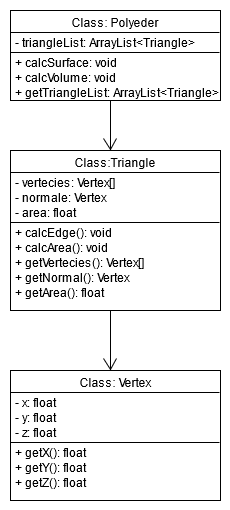
\includegraphics[height=.5\textheight]{PolyederUML}
	\end{center}

	\section*{Argumentation/Beschreibung}
	Um ein Polyeder zu modellieren, wurden drei Klassen entworfen, die zusammengesetzt ein Polyeder beschreiben. Da ein Polyeder nur aus Dreiecken in der Standard Triangulation Language (STL) bestehen kann, ist die Klasse Polyeder, die einen Polyeder repräsentiert, in einer Kompositionsbeziehung mit der Klasse Triangle, die wiederum ein Dreieck im Modell repräsentiert. Dieselbe Beziehung steht auch zwischen einem Dreieck und seinem Eckpunkten den Vertices, die Vertices werden mit der Klasse Vertex repräsentiert. Die Klasse Vertex besitzt die drei Attribute x, y und z. Diese drei Attribute speichern die jeweiligen Achsenpositionen eines Dreidimensionalen Koordinatensystem, die ein Vertex besitzt. In der Klasse Triangle werden folgende Attribute bestimmt. Das Attribut vertices speichert ein Array an Vertices, die für den Aufbau eines Dreiecks benötigt werden. Das Attribut normale ist vom Typ Vertex und speichert die Normale des Dreiecks, die laut Definition benötigt wird. Als letztes Attribut wird area festgelegt. Das Attribut speichert den Flächeninhalt eines Dreiecks als Float. Das Attribut triangleList in der Klasse Polyeder wird benötigt, da ein Polyeder nur aus Dreiecken bestehen kann und diese abgespeichert werden müssen. Dafür ist das Attribut triangleList eine ArrayList, die nur Objekte vom Typ Triangle aufnehmen kann. Die Collection ArrayList wurde gewählt, da ein Polyeder aus vielen verschiedenen Dreiecken bestehen kann und ein statischer Datentyp wie z.B. ein normales Array nicht flexibel genug ist. Des Weiteren besitzt die Klasse Polyeder die zwei Attribute surface und volume. Diese speichern die Werte für die Oberfläche und für das Volumen. Alle Attribute in den drei Klassen sind private, damit die Datenkapselung umgesetzt wird. Um auf die Werte zuzugreifen oder diese zu verändern wurden dafür Methoden deklariert. 
	Die Klasse Polyeder besitzt die privaten Methoden calcSurface() und calcVolume(). Diese werden zur Berechnung der Oberfläche und des Volumen eines Polyeders benutzt. Zudem existieren die öffentlichen Methoden getSurface() und getVolume(), die die Werte für die Oberfläche und für das Volumen zurückgeben. Au\ss erdem besitzt die Klasse Polyeder die öffentliche Methode getTriangleList(), die die ArrayList für die gespeicherten Dreiecke zurück gibt.  
	Die Klasse Triangle besitzt folgende Methoden  calcEdge(p1: Vertex, p2: Vertex), calcArea(), getVertices(), getArea(), getNormal(). Die Methode calcEdge(p1: Vertex, p2: Vertex) ist Privat und berechnet die Kante zwischen den beiden Vertices p1 und p2. Diese Methode wird genutzt in der privaten calcArea() Methode um mit den zurückgegebenen Wert den Flächeninhalt des Dreiecks zu berechnen. Die öffentliche Methode  getVertices() gibt das gespeicherte Array von Vertices zurück. Die öffentliche Methode getNormal() gibt die gespeicherte Normale zurück. Die öffentliche  Methode getArea() gibt den gespeicherten Wert vom Flächeninhalt zurück. Die Klasse Vertex implementiert die öffentlichen Methoden getX(), getY(), getZ(). Diese geben die jeweiligen gespeicherten x, y und z Positionen eines Vertex zurück. Alle Klassen besitzen einen Konstruktor, indem die privaten Berechnungsmethoden aufgerufen werden und die Startattribute gesetzt werden.
	
	
\end{document}
